\documentclass[../main.tex]{subfiles}
\graphicspath{{\subfix{../images/}}}
\begin{document}
\subsection*{Answers - Integration by parts - DI method (page \pageref{DI Method})}
\label{DI method answers}
\begin{enumerate}
    \item \(\int x^2\sin{(2x)}\, dx\)
    
    \begin{figure}[h]
    \setlength\parindent{30pt}
        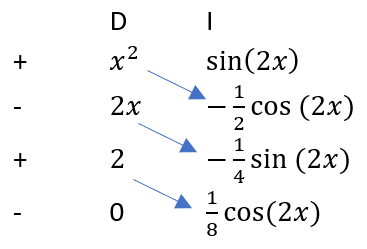
\includegraphics[width=0.25\linewidth]{images/di_a1.png}
    \end{figure}
    
    Stop is reached when we get zero in the D row.

    \(\int x^2\sin{(2x)}\, dx=-\frac{x^2}{2}\cos{(2x)}+\frac{x}{2}\sin{(2x)}+\frac{1}{4}\cos{(2x)}+c\)

    \item \(\int e^x \cos{(x)}\, dx\)
    
    \begin{tabular}{ c c c }
       & D & I \\ 
     +  & $e^x$ &$\cos{x}$ \\  
     - & $e^x$ & $\sin{x}$\\
      + & $e^x$ & $-\cos{x}$ \\  
    \end{tabular}

    The third row is a “repeat” of the first, so we can stop now. The integral is diagonal products plus the integral of the final row product.

    \(\int e^x \cos{(x)}\, dx = e^x\sin{(x)}+e^x\cos{(x)}-\int e^x\cos{(x)}\,dx\)

    \(2\int e^x \cos{(x)}\, dx= e^x\sin{(x)}+e^x\cos{(x)}\)

    \(\int e^x \cos{(x)}\, dx=\frac{e^x\sin{(x)}+e^x\cos{(x)}}{2}+c\)
    
    \item \(\int (\ln{(x)})^2\, dx\)
    
    \begin{tabular}{ c c c }
       & D & I \\ 
     +  & $\ln{(x)})^2$ &$1$ \\  
     - & $\frac{2\ln{x}}{x}$ & $x$\\ 
    \end{tabular}

    Since the product of the second row can (relatively) easily be integrated, the integral will be:

    \(\int (\ln{(x)})^2\, dx=x\ln{(x)})^2-\int 2\ln{x}\, dx\)

    Using the DI method again for this:

    \begin{tabular}{ c c c }
       & D & I \\ 
     +  & $2\ln{x}$ &$1$ \\  
     - & $\frac{2}{x}$ & $x$\\ 
    \end{tabular}

    The product of the second row can be integrated so we stop, giving us:

    \(2\ln{x}\, dx=2x\ln{x}-\int 2\,dx=2x\ln{x}-2x\)

    Therefore, our final integral is:

    \(\int (\ln{(x)})^2\, dx=x(\ln{(x)})^2-2x\ln{x}+2x+c\)

    \item \(\int \sin^3{(x)}\,dx\)
    
    \begin{tabular}{ c c c }
       & D & I \\ 
     +  & $\sin^2{(x)}$ &$\sin{(x)}$ \\  
     - & $2\sin{(x)}\cos{(x)}$ & $-\cos{(x)}$\\ 
    \end{tabular}

    The product of the second row integrates easily so we stop:

    \(\int 2\sin{(x)}\cos^2{(x)}\, dx=-\frac{2}{3}\cos^3{(x)}\)

    Therefore, our final integral is:

    \(\int \sin^3{(x)}\,dx=-\sin^2{(x)}\cos{(x)}-\frac{2}{3}\cos^3{(x)}+c\)

    \item \(\int \frac{\ln{(x)}}{x^2}\, dx\)
    
    \begin{tabular}{ c c c }
       & D & I \\ 
     +  & $\ln{x}$     &$\frac{1}{x^2}$ \\  
     - & $\frac{1}{x}$   & $-\frac{1}{x}$\\ 
    \end{tabular}

    The product of the second row is easy to integrate so we stop:

    \(\int \frac{\ln{(x)}}{x^2}\, dx=-\frac{\ln}{x}-\int -\frac{1}{x^2}\, dx\)
    
    \(\int \frac{\ln{(x)}}{x^2}\, dx=-\frac{\ln}{x}+\int \frac{1}{x^2}\, dx\)

    \(\int \frac{\ln{(x)}}{x^2}\, dx=-\frac{\ln}{x}-\frac{1}{x}+c\)

    \item \(\int 4x\cos{(2-3x)}\, dx\)
    
    \begin{tabular}{ c c c }
       & D & I \\ 
     +  & $4x$     &$\cos{(2-3x}$ \\  
     - & $4$   & $-\frac{1}{3}\sin{(2-3x)}$\\ 
     + & $0$   & $-\frac{1}{9}\cos{(2-3x)}$\\
    \end{tabular}

    Stop because we reach zero in the D column, so the integral is:

    \(\int 4x\cos{(2-3x)}\, dx=-\frac{4x}{3}\sin{(2-3x)}+\frac{4}{9}\cos{(2-3x)}+c\)

    \item \(\int e^{-x}\cos{(x)}\, dx\)
    
    \begin{tabular}{ c c c }
       & D & I \\ 
     +  & $e^{-x}$     &$\cos{(x)}$ \\  
     - & $-e^{-x}$   & $\sin{(x)}$\\ 
     + & $e^{-x}$   & $-\cos{(x)}$\\
    \end{tabular}

    The third row repeats, so we stop:

    \(\int e^{-x}\cos{(x)}\, dx=e^{-x}\sin{(x)}-e^{-x}\cos{(x)}+\int e^{-x}\times -\cos{(x)}\, dx\)

    \(\int e^{-x}\cos{(x)}\, dx=e^{-x}\sin{(x)}-e^{-x}\cos{(x)}-\int e^{-x}\cos{(x)}\, dx\)

    \(2\int e^{-x}\cos{(x)}\, dx=e^{-x}\sin{(x)}-e^{-x}\cos{(x)}x\)

    \(\int e^{-x}\cos{(x)}\, dx=\frac{e^{-x}}{2}(\sin{(x)}-\cos{(x)})+c\)
      
\end{enumerate}
\end{document}